\documentclass[a4paper,11pt]{article}
\usepackage[margin=25mm]{geometry}
\usepackage{fontspec,unicode-math,amsmath,booktabs,graphicx,hyperref}
\setmainfont{STIXGeneral}\setmathfont{STIX Two Math}\hypersetup{hidelinks}
\setlength{\parindent}{0pt}\setlength{\parskip}{4pt}\setlength{\emergencystretch}{2em}
\title{Locally projective quotients: complete written costs}
\author{Human Compression project}\date{Private numerical candidate; distinct review pending}
\begin{document}\raggedright\begin{center}{\Large\bfseries Locally projective quotients: complete written costs}\\[4pt]Human Compression project\\{\small Private numerical candidate; distinct review pending}\end{center}
Two originals remain distinct: L084 is the complete two-page 2006 publisher
erratum, and L095 is the full fifteen-page July 2003 arXiv v1. The accepted
replacement recovers their corrected principal contracts, with all 52 source
dispositions and all 145 historical rows retained. No unseen journal edition
or corrected source text is substituted in the numerator.

\section*{Written papers}
The primary unit is the number of non-whitespace characters in NFC, after exact
running furniture removal and the accepted visible-symbol calibration.
Titles, abstract, addresses, version banner, tables and references remain.
\begin{center}\begin{tabular}{@{}lrr@{}}\toprule Complete document & Pages & Characters\\\midrule
L084 original & 2 & 2,071\\
L095 original & 15 & 24,419\\
Common proof & 7 & 19,533\\
Common census tables & 5 & 5,965\\
L084 application & 2 & 4,857\\
L095 application & 3 & 7,109\\\midrule
Combined originals & 17 & 26,490\\
Whole common and applications & 17 & 37,464\\\bottomrule\end{tabular}\end{center}
The common bundle includes the complete marked-group, geometry and census
proofs. Neither application borrows an unpaid proof from its sibling or another
topic. Writing $U^*=U+\mathrm{tables}$, the combined written comparison is
\[\frac{c(L084)+c(L095)}{c(U^*)+c(A_1)+c(A_2)}=\frac{26490}{37464}=0.707079.\]
The written replacement is longer by 10,974 characters in this coordinate.
A factor below one records that increase; it is not a compression gain.
\begin{center}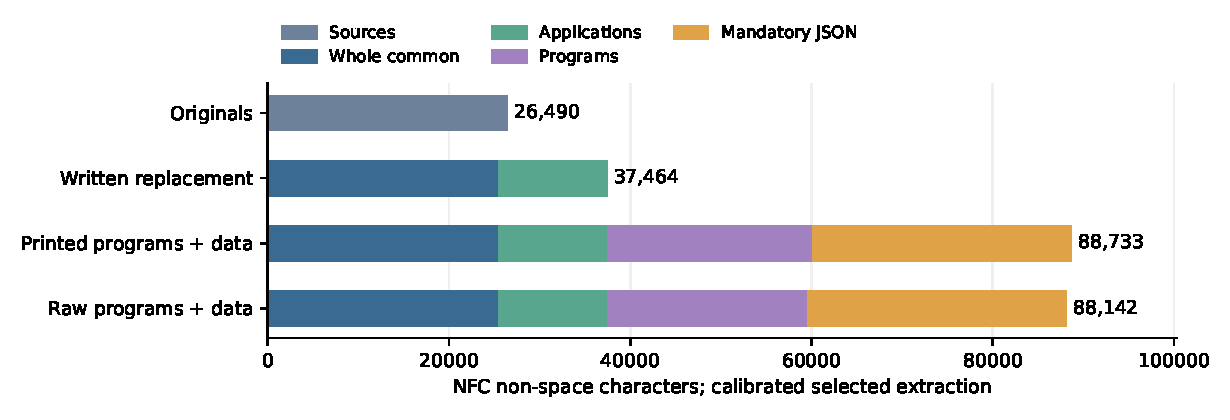
\includegraphics[width=\linewidth]{costs.pdf}\end{center}
\newpage
\section*{Including the complete programs and data}
All six complete mathematical programs are required finite computations.
Their six-page printed appendix costs 22,695 characters; the full raw
alternative costs 22,104. In \emph{both} cases the entire required
\texttt{source\_tables.json} adds 28,574 characters (39,150 raw bytes).
Its 145 rows are used in historical reconciliation, not subgroup enumeration.
The printed code is not a substitute for these data. Thus the two alternatives are
\[\frac{c(L084)+c(L095)}{c(U^*)+c(A_1)+c(A_2)+c(\mathrm{printed\ programs})+c(\mathrm{data})}=\frac{26490}{88733}=0.298536,\]
\[\frac{c(L084)+c(L095)}{c(U^*)+c(A_1)+c(A_2)+c(\mathrm{raw\ programs})+c(\mathrm{data})}=\frac{26490}{88142}=0.300538.\]
Neither row adds both code representations or prunes any file or data field.

\section*{After acquiring the whole common theory, programs and data}
The conditional comparisons are source/application only after that acquisition:
\[\frac{c(L084)}{c(A_1)}=\frac{2071}{4857}=0.426395,\qquad \frac{c(L095)}{c(A_2)}=\frac{24419}{7109}=3.434942.\]
The prior known acquisition is 25,498 for the whole common bundle, plus the
complete code and 28,574 for data: 76,767 using printed code, or 76,176
using raw code. Retained external inputs are also prerequisites; their full costs
are unknown. These conditional factors do not replace the combined comparison.
\begin{center}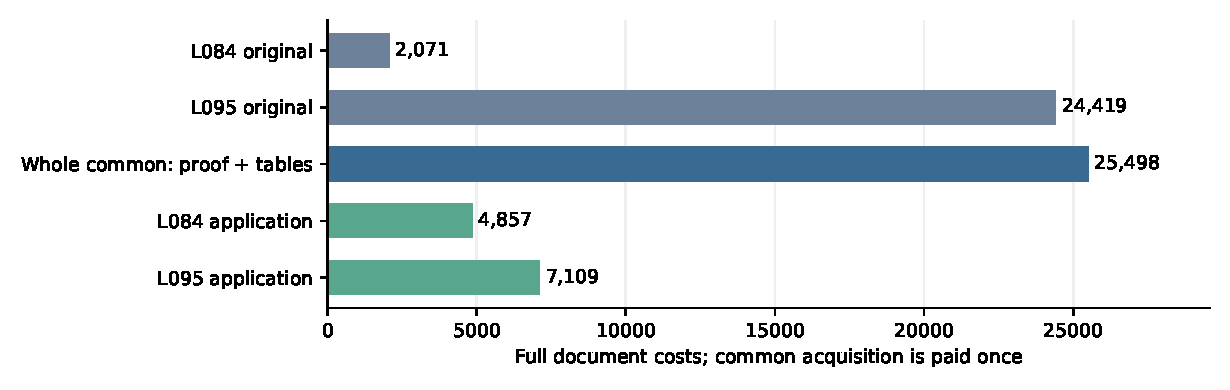
\includegraphics[width=\linewidth]{documents.pdf}\end{center}

\section*{Separate costs and limits}
The six raw programs total 24,255 bytes. Three operational drivers total 32,220
raw bytes (29,370 primary characters). Eleven regenerated outputs total
3,470,182 bytes, including the complete computed subgroup representatives.
They remain separately inventoried; outputs generated in the same computation
are not charged again as independent enumeration inputs. No output-text metric
or formal proof cost is inferred from storage bytes. There are no Lean files or
declarations in this edition.

Classical local geometry and polytope correspondences, named finite groups,
and exact GAP/ACE/NetworkX algorithms remain retained inputs. Thirteen selected
runtime/model pins do not measure their full implementations or proofs.
Those costs, historical software, graphics/layout and full formalization remain
unknown, not zero. The unavailable historical \texttt{g.txt} is not used.
No new mathematical, source, question or formal credit is claimed.
\newpage
\section*{Metric and extraction sensitivity}
All 30 coordinates keep the same complete boundary. ``Printed+data'' and
``Raw+data'' include the full mandatory JSON; the two conditional columns
assume all prior acquisition specified above. The table rounds display only;
JSON and CSV retain all 150 exact fractions.

{\fontsize{8.4}{10}\selectfont \par\vspace{6pt}\textbf{Untrimmed extraction}\par\smallskip\begin{tabular}{@{}llrrrrr@{}}\toprule Unit & Form & Written & Printed+data & Raw+data & L084 cond. & L095 cond.\\\midrule Whitespace tokens & NFC & 0.819493 & 0.527655 & 0.531570 & 0.426966 & 4.646223 \\
Alphanumeric runs & NFC & 0.780686 & 0.388078 & 0.390559 & 0.448313 & 4.349927 \\
Non-space characters & NFC & 0.707959 & 0.298966 & 0.300990 & 0.431159 & 3.436445 \\
Collapsed characters & NFC & 0.727686 & 0.327183 & 0.329441 & 0.430411 & 3.628196 \\
Collapsed UTF-8 bytes & NFC & 0.721622 & 0.331488 & 0.333729 & 0.428963 & 3.628085 \\
Whitespace tokens & NFKC & 0.820114 & 0.528056 & 0.531973 & 0.426966 & 4.649963 \\
Alphanumeric runs & NFKC & 0.780686 & 0.388078 & 0.390559 & 0.448313 & 4.349927 \\
Non-space characters & NFKC & 0.709770 & 0.299744 & 0.301774 & 0.432393 & 3.445444 \\
Collapsed characters & NFKC & 0.729286 & 0.327914 & 0.330177 & 0.431454 & 3.636364 \\
Collapsed UTF-8 bytes & NFKC & 0.744535 & 0.335913 & 0.338219 & 0.432451 & 3.720859 \\\bottomrule\end{tabular}
\par\vspace{6pt}\textbf{Exact furniture removed}\par\smallskip\begin{tabular}{@{}llrrrrr@{}}\toprule Unit & Form & Written & Printed+data & Raw+data & L084 cond. & L095 cond.\\\midrule Whitespace tokens & NFC & 0.818737 & 0.527025 & 0.530685 & 0.422297 & 4.645427 \\
Alphanumeric runs & NFC & 0.779734 & 0.387339 & 0.389675 & 0.442748 & 4.348496 \\
Non-space characters & NFC & 0.707079 & 0.298536 & 0.300538 & 0.426395 & 3.434942 \\
Collapsed characters & NFC & 0.726801 & 0.326690 & 0.328906 & 0.425662 & 3.626510 \\
Collapsed UTF-8 bytes & NFC & 0.720769 & 0.331007 & 0.333207 & 0.424289 & 3.626458 \\
Whitespace tokens & NFKC & 0.819360 & 0.527426 & 0.531089 & 0.422297 & 4.649175 \\
Alphanumeric runs & NFKC & 0.779734 & 0.387339 & 0.389675 & 0.442748 & 4.348496 \\
Non-space characters & NFKC & 0.708890 & 0.299315 & 0.301322 & 0.427630 & 3.443944 \\
Collapsed characters & NFKC & 0.728402 & 0.327421 & 0.329642 & 0.426706 & 3.634684 \\
Collapsed UTF-8 bytes & NFKC & 0.743671 & 0.335426 & 0.337690 & 0.427731 & 3.719253 \\\bottomrule\end{tabular}
\par\vspace{6pt}\textbf{Furniture removed and visible symbols calibrated}\par\smallskip\begin{tabular}{@{}llrrrrr@{}}\toprule Unit & Form & Written & Printed+data & Raw+data & L084 cond. & L095 cond.\\\midrule Whitespace tokens & NFC & 0.818737 & 0.527025 & 0.530685 & 0.422297 & 4.645427 \\
Alphanumeric runs & NFC & 0.779611 & 0.387278 & 0.389614 & 0.441658 & 4.348496 \\
Non-space characters & NFC & 0.707079 & 0.298536 & 0.300538 & 0.426395 & 3.434942 \\
Collapsed characters & NFC & 0.726801 & 0.326690 & 0.328906 & 0.425662 & 3.626510 \\
Collapsed UTF-8 bytes & NFC & 0.724142 & 0.332556 & 0.334766 & 0.426687 & 3.643151 \\
Whitespace tokens & NFKC & 0.819360 & 0.527426 & 0.531089 & 0.422297 & 4.649175 \\
Alphanumeric runs & NFKC & 0.779611 & 0.387278 & 0.389614 & 0.441658 & 4.348496 \\
Non-space characters & NFKC & 0.708890 & 0.299315 & 0.301322 & 0.427630 & 3.443944 \\
Collapsed characters & NFKC & 0.728402 & 0.327421 & 0.329642 & 0.426706 & 3.634684 \\
Collapsed UTF-8 bytes & NFKC & 0.743714 & 0.335446 & 0.337709 & 0.428077 & 3.719253 \\\bottomrule\end{tabular}}

The untrimmed coordinate retains every extracted character, including running
furniture. Selected variants remove only the exact erratum running header and
isolated page numbers. Eight actual font classes receive 61 occurrence-bound
repairs: calligraphic capitals, a correspondence envelope, proof-end squares
and mapsto tails. A tail remains separate from its adjacent arrow. Printed
hyphens remain literal; NFC and NFKC are distinct sensitivities.

The source’s incorrect historical counts are not changed by calibration.
L095’s table rules are inline images. This is a full-document extractable-text
comparison, not a complete measure of graphical construction or intrinsic proof
complexity. The numerical author also authored the inputs; the accepted input
review was distinct. These new calculations require their own independent
review. No source extraction, GAP, census or Lean execution was repeated here.
\end{document}
